% !TeX program = pdflatex
\documentclass[border=6pt]{standalone}
\usepackage{amsmath}
\usepackage{tikz}
\usetikzlibrary{arrows.meta, positioning, calc}

\definecolor{MediumRed}{rgb}{0.925, 0.345, 0.345}
\definecolor{MediumGreen}{rgb}{0.37, 0.7, 0.66}
\definecolor{MediumBlue}{rgb}{0.015, 0.315, 0.45}
\definecolor{DarkBlue}{rgb}{0.05, 0.15, 0.35}

\begin{document}
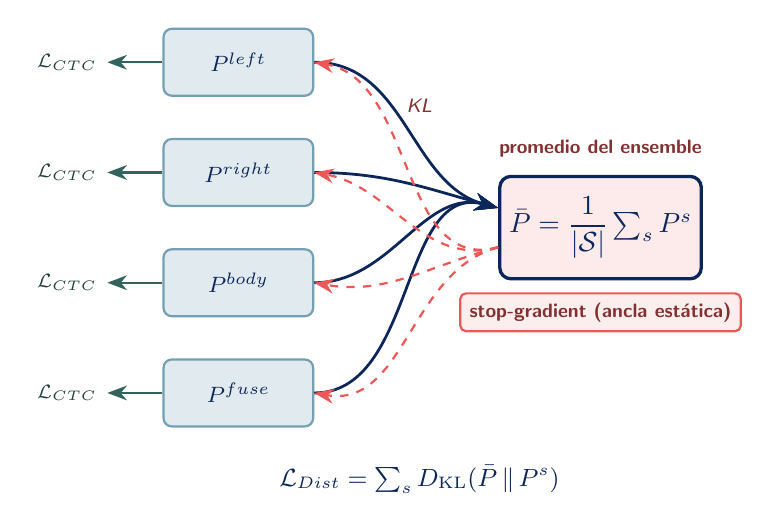
\begin{tikzpicture}[
    font=\sffamily,
    head/.style={draw=MediumBlue!55, thick, rounded corners=3pt, fill=MediumBlue!12,
        text=DarkBlue, align=center, minimum width=1.9cm, minimum height=0.85cm,
        font=\sffamily\footnotesize},
    flow/.style={-{Stealth[length=3mm]}, line width=1pt, DarkBlue},
]

% cabezas
\node[head] (l) at (0,2.1) {$P^{left}$};
\node[head] (r) at (0,0.7) {$P^{right}$};
\node[head] (b) at (0,-0.7) {$P^{body}$};
\node[head] (f) at (0,-2.1) {$P^{fuse}$};

% CTC a la izquierda
\foreach \n in {l,r,b,f}
    \draw[-{Stealth[length=2.5mm]}, MediumGreen!55!black, thick]
        (\n.west) -- ++(-0.7,0) node[left, font=\sffamily\scriptsize, text=MediumGreen!35!black] {$\mathcal{L}_{CTC}$};

% promedio
\node[draw=DarkBlue, very thick, rounded corners=4pt, fill=MediumRed!12, text=DarkBlue,
      align=center, minimum width=2.2cm, minimum height=1.3cm] (avg) at (4.6,0) {$\bar{P}=\dfrac{1}{|\mathcal S|}\sum_s P^{s}$};
\node[font=\sffamily\scriptsize\bfseries, text=MediumRed!55!black, above=0.1cm of avg]
    {promedio del \emph{ensemble}};

\foreach \n in {l,r,b,f}
    \draw[flow] (\n.east) to[out=0,in=165] ($(avg.west)+(0,0.25)$);

% stop gradient
\node[draw=MediumRed, thick, rounded corners=2pt, fill=MediumRed!10, text=MediumRed!55!black,
      font=\sffamily\scriptsize\bfseries, below=0.15cm of avg] (sg) {\textit{stop-gradient} (ancla estática)};

% KL de vuelta a cada cabeza
\foreach \n in {l,r,b,f}
    \draw[-{Stealth[length=2.5mm]}, MediumRed, thick, dashed]
        ($(avg.west)+(0,-0.25)$) to[out=195,in=-10] (\n.east);
\node[font=\sffamily\scriptsize\itshape, text=MediumRed!55!black] at (2.3,1.55) {KL};

\node[font=\sffamily\small\bfseries, text=DarkBlue] at (2.3,-3.2)
    {$\mathcal{L}_{Dist}=\sum_{s} D_{\mathrm{KL}}(\bar P \,\|\, P^{s})$};

\end{tikzpicture}
\end{document}
